\documentclass{report}

\usepackage[margin=1in]{geometry}
\usepackage{amsmath,amsthm,amssymb}
\usepackage{enumitem}
\usepackage{graphicx}
\usepackage{caption}
\usepackage{mathtools}
\renewcommand{\familydefault}{\sfdefault}
\begin{document}
% ------------------------------------------ %
%                 START HERE                 %
% ------------------------------------------ %
\title{CS5785 Homework 1\\
\large{
    Applied Machine Learning
}
}


\author{
	Vijay Pillai\\
	Thomas Matecki}
\maketitle
\section*{Programming Exercises}

\begin{enumerate}
	\item Digit Tokenizer
	\begin{enumerate}[label=(\alph*)]
		\item 
		Training and test data are located in files \textit{train.csv} and \textit{test.csv} respectively. The training data comprises 42000 images and the test data comprises 28000 images.

		\item Figure 1 is one of each digit(0-9) displayed as a 28 by 28 pixel grid.  
		\begin{center}
		\captionof{figure}{}
%		\includegraphics[width=12cm]{one_of_each_digit.png}
		\end{center}
		Alternatively, the digit images can be plotted as one dimensional vectors (length = 784).
		\begin{center}
		\captionof{figure}{}
%		\includegraphics[width=12cm]{Figure_2.png}
		\end{center}
		\newpage
		\item The distribution of digits within the training data is nearly uniform.
		\begin{center}
%		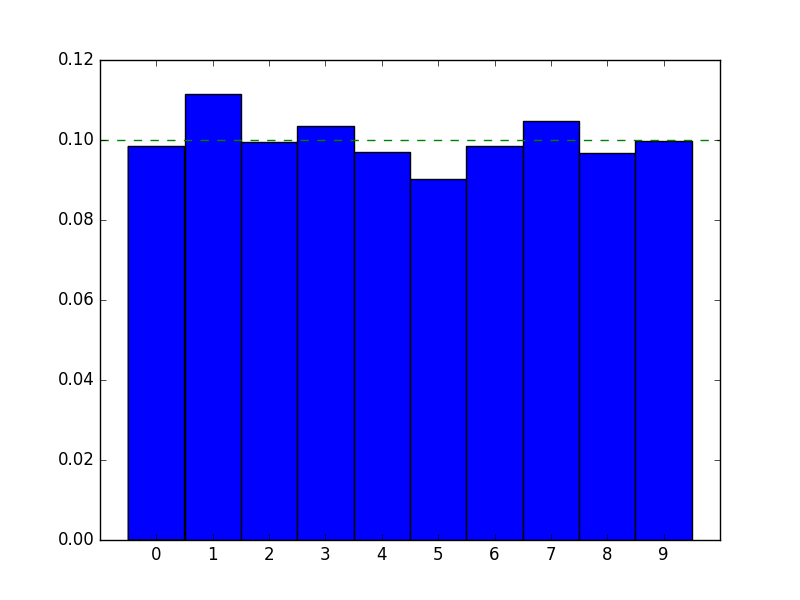
\includegraphics{distrib.png}
		\end{center}	
		\item
	\end{enumerate}
	\item The Titanic Disaster
	\begin{enumerate}[label=(\alph*)]
		\item Pro
		\item 
	\end{enumerate}
	
\end{enumerate}

\section*{Written Exercises}	
\begin{enumerate}
	\item Based on the defintions of variance:\\
	\centerline{$var(X) = E[(X - E[X])^2]$}
	and covariance,\\
	\centerline{$cov(X) = E[(Y - E[Y])(X - E[X])$}
	we have:
	\begin{align*}
    var[X-Y] &= E[( X - Y - E[X - Y])^2]  \\
    	 	 &= E[( X - Y - E[X] - E[Y])^2] \\
    	 	 &= E[( X - E[X]) - (Y - E[Y]) )^2] \\
    	 	 &= E[( X - E[X])^2 - 2E[(Y - E[Y])(X - E[X])] + E[(Y - E[Y])^2]] \\
    	 	 &= var(X) + var(Y) - 2E[(Y - E[Y])(X - E[X])] \\
    	 	 &= var(X) + var(Y) - 2cov(X,Y ) \\
    \end{align*}
	\item Letting event R be a positive test result, and event D be the occurence of a defective widget, we have...
	\begin{align*}
	     & P(D) = \frac{1}{100,000} \\
	     & P(R \vert D) = .95  \\
	     & P(\lnot R \vert \lnot D) = .95 \\
	 \end{align*}
	    ...and therefore...
	    \begin{align*}
	     & P(\lnot D) 				= 1 - \frac{1}{100,000} = \frac{99,999}{100,000} \\
	     & P(\lnot R \vert 		D) 	= 1-  P(R \vert D) =.05  & 
	     \text{(because $R \cap \lnot R = \emptyset$)}\\
	     & P(R 		\vert \lnot D) 	= .05  \\
	 	\end{align*}
	 	Additionally, the probability of a positive test result is the sum of the probabilities of a  defective widget testing positive and a non-defective widget testing positive; i.e.,
	 	\begin{align*}
	 	 P(R) 	&= P(R \cap D) + P(R \cap \lnot D)\\
	 	 		&= P(R \vert D)P(D) + P(R \vert \lnot D)P(\lnot D) \\
	 	 		&= (.95)\frac{1}{100,000} + (.05)\frac{99,999}{100,000} 
	 	 		 = \frac{.95}{100,000} + \frac{4999.95}{100,000} 
	 	 		 = \mathbf{\frac{5000.9}{100,000}}\\
	    \end{align*}
	    
	     
	    \begin{enumerate}[label=(\alph*)]
		\item Given a positive test result, the probability the widget is actually defective is:
	 	\begin{align*}
	 	 P(D \vert R)	&= \frac{P(R \vert D)P(D)}{P(R)} & \text{(bayes rule)} \\
	 	 				&= \frac{\frac{.95}{100,000}}{\frac{5000.9}{100,000}}
	 	 				 = \mathbf{0.000189966}
	    \end{align*}
		\item The probability a widget is not defective and tests positive is:
		\begin{align*}
		P(R \cap \lnot D) = P(R \vert \lnot D)P(\lnot D) 	&= (.05)\frac{99,999}{100,000} \\
															&= 0.0499995
		\end{align*}
		The probability a widget is defective and does not test positive is:
		\begin{align*}
		P(\lnot R \cap D) = P(\lnot R \vert  D)P(D) 	&= \frac{.05}{100,000} \\
														&= 0.0000005
		\end{align*}
		Therefore 499995 non-defective widgets are thrown out and 5 defective widgets are shipped per year.
		\end{enumerate}
		
\end{enumerate}

\end{document}
 